\chapter{XyloDensMap}

In France, national estimates of forest biomass and carbon stocks have so far relied on wood density values derived from an unpublished dataset, compiled from a literature review conducted by Jean-Luc Dupouey (INRAE) as part of the CARBOFOR project \parencite{Loustau2004}. Some of these values originate from a 170-year-old source \parencite{Mathieu1855}, updated to provide a single average value per species, covering around 50 species. However, these estimates are based on small and unbalanced samples—typically fewer than 10 mature trees per species and do not reflect the diversity of conditions found in French forests, particularly in terms of species, tree size, and growth conditions. \\

To address the lack of precise and comprehensive data on wood density for forest species in mainland France, the Xylo\-Dens\-Map project was launched in 2015 through a collaboration between INRAE and IGN. The resulting open dataset, Xylo\-Dens\-Map, includes individual wood density measurements from \num{110763} wood cores taken at breast height across metropolitan France. These data were obtained by combining the spatially systematic sampling design of the French National Forest Inventory (NFI) with a high-throughput method for measuring wood density using X-ray computed tomography \parencite{Freyburger2009,Jacquin2019}. Due to the systematic nature of the IFN's annual sampling framework \parencite{Bontemps2024,Bouriaud2023}, the Xylo\-Dens\-Map dataset is representative of French forests, particularly in terms of species diversity and tree size. \\

All details regarding the sampling design, sample processing, and wood density measurement in Xylo\-Dens\-Map are provided in the corresponding data paper \parencite{Cuny2025}. A second publication on wood density modeling in France using the Xylo\-Dens\-Map dataset is currently under review at Biogeosciences, with the article already available as a preprint \parencite{Cuny2025_a}. This work compares the application of different methods (average species coefficients, more detailed linear models incorporating tree size and climatic conditions, random forest) to simulate wood density in IFN data, and discusses the influence of the chosen method on estimating total aboveground biomass stocks at multiple scales in France. The publication thus already includes simulations of wood density across the entire NFI framework (see Fig.  \ref{fig::map_density})---a necessary step for calculating biomass and carbon stocks and fluxes at different scales in France---and may serve as a basis for discussion to define the method to be used for simulating wood density in the NFI dataset.
\begin{marginfigure}[-4cm]
	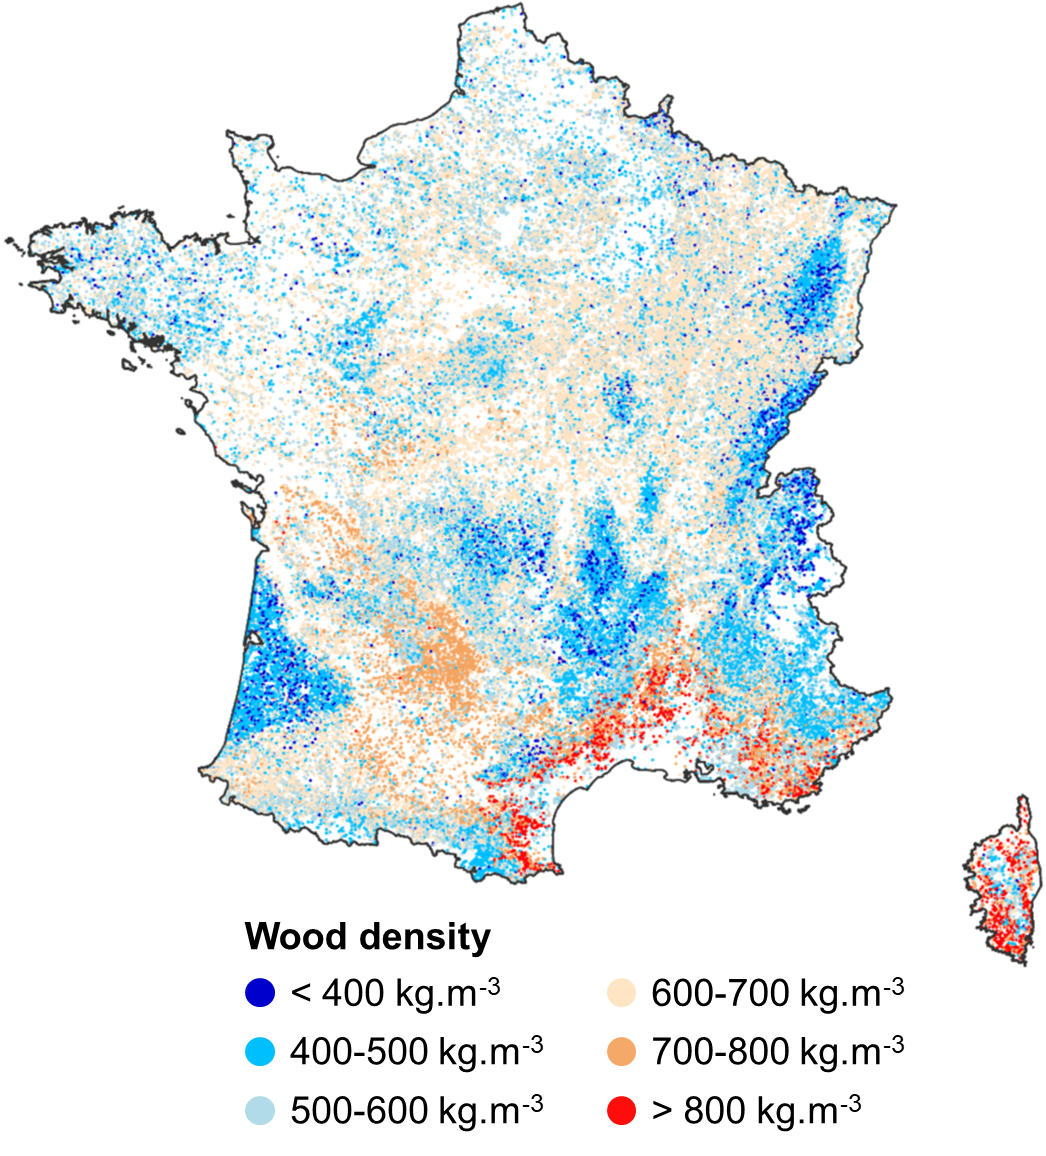
\includegraphics[width = \marginparwidth]{./Figures/map_density.png}
	\caption{Map of community-wide mean wood density in mainland France on each forest plot inventoried by the French \NFI{} between2005 and 2022.\label{fig::map_density}}
\end{marginfigure}


\chapter{Root volume and wood carbon content}

While actions regarding aboveground volumes (stem wood and total aerial biomass) and wood density are already underway, aspects related to root volume and carbon content in wood remain less explored at this stage. Unlike the evaluation of or wood density, the IGN does not currently have datasets that allow for the analysis of root volumes or wood carbon content. For these aspects, a different approach will be implemented, involving a literature review to assess the current state of knowledge. \\

The objective will be to determine whether the current assumptions used in the IGN method---namely, a root expansion coefficient by botanical class (1.28 for broadleaves and 1.30 for conifers) and a single carbon content coefficient (0.475)---are still relevant in light of current knowledge, or whether they could be improved to better reflect natural variability. The literature review will be complemented by discussions with expert researchers in these fields, such as those at the INRAE center in Champenoux. \\

An internship was already conducted during the summer of 2025 on this topic. It helped identify a number of bibliographic references for each aspect. Regarding wood carbon content, many articles have recently been published, and a global database was even compiled through a literature review \parencite{Doraisami2022}. This database includes carbon content values for several species found in French forests. As for root volume, an interview was conducted with Frédéric Danjon, a root specialist at INRAE, which provided access to numerous relevant references on root volume. A synthesis of the various identified references for each aspect now needs to be carried out. \\

Should the assumptions regarding root volume and carbon content be revised, an analysis and documentation of the impact of these revisions on carbon estimates will be undertaken.